\documentclass[border=10pt]{standalone}

\usepackage{tikz}
\usepackage{tikzsymbols}
\usetikzlibrary{calc,patterns,shapes.geometric}

\def\centerarc[#1](#2)(#3:#4:#5){\draw[#1] ($(#2)+({#5*cos(#3)},{#5*sin(#3)})$) arc (#3:#4:#5);}

\begin{document}
	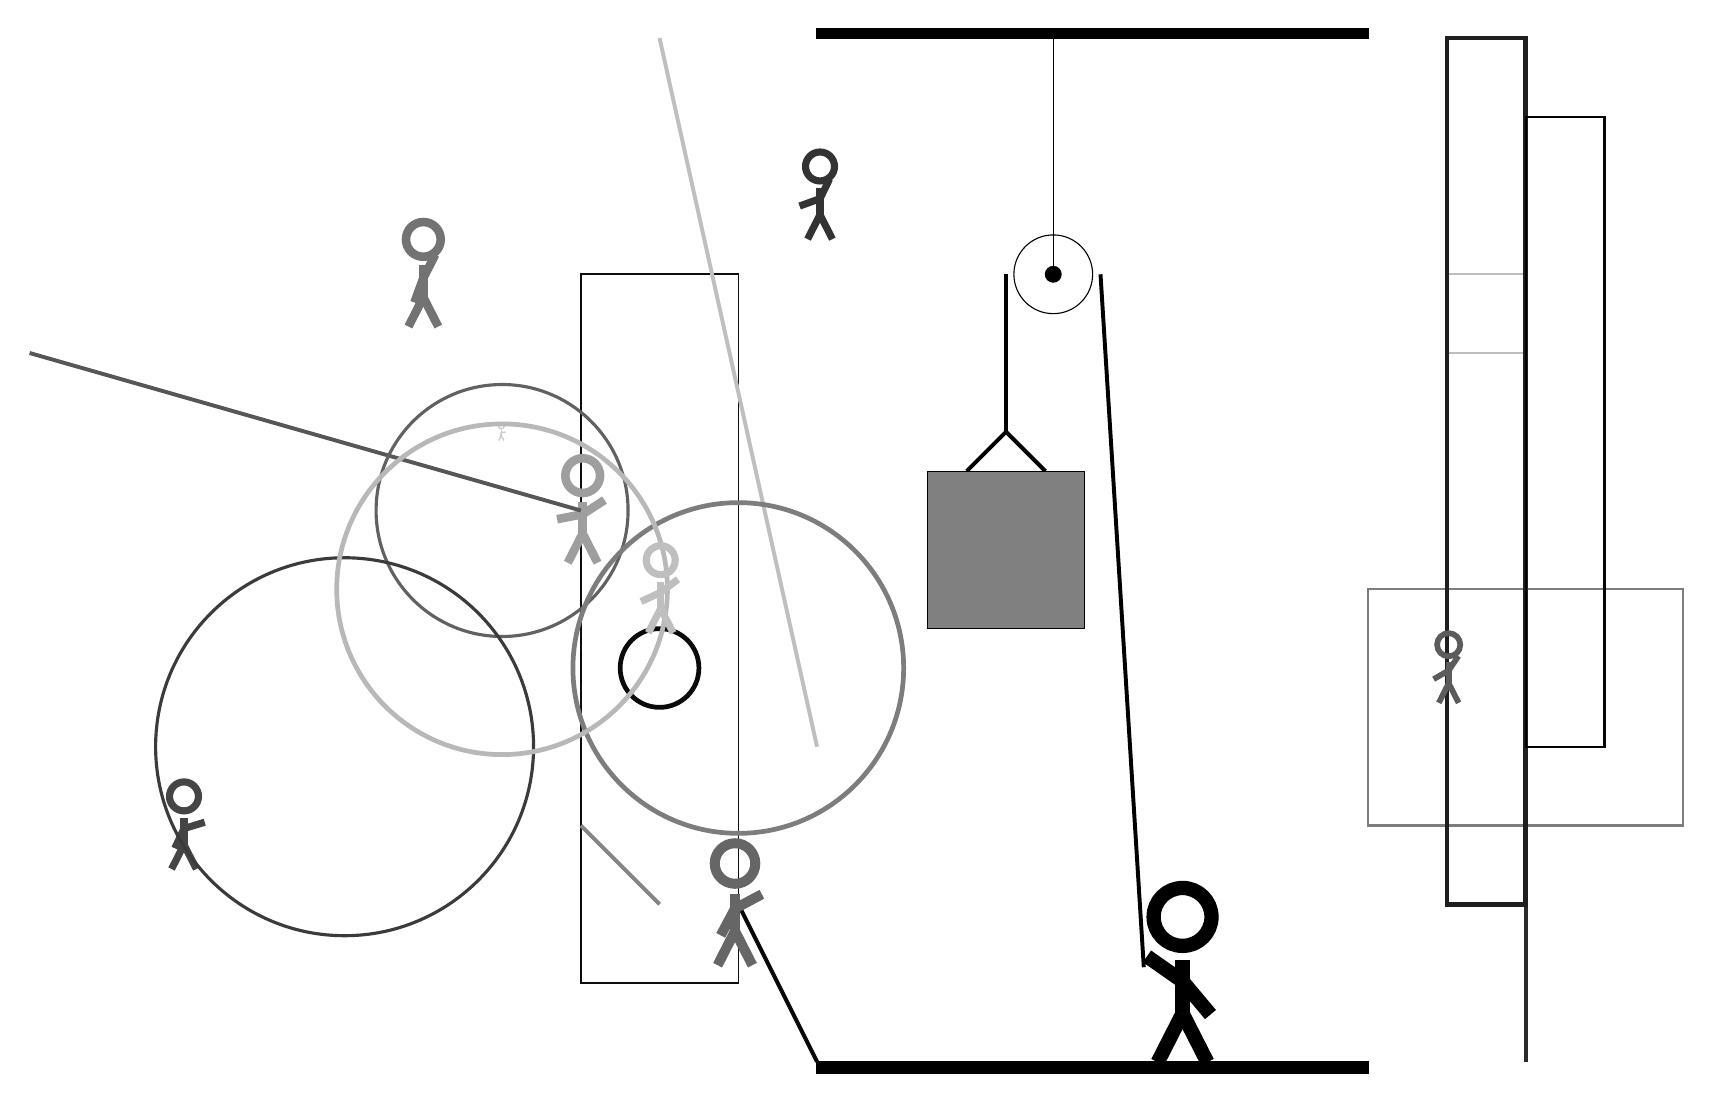
\begin{tikzpicture}
		%%%%% START %%%%%
		
		\draw[fill=black] (-2, 10) rectangle (5, 10.125);
		
		\draw (1, 7) circle (0.5);
		\draw[fill=black] (1, 7) circle (0.1);
		\draw (1, 10) -- (1, 7);
		
		\draw[line width=0.5mm] (-0.1, 4.5) -- (0.4, 5.0) -- (0.9, 4.5);
		\draw[fill=black!50] (-0.6, 4.5) rectangle (1.4, 2.5);
		
		\draw[line width=0.5mm] (0.4, 7) -- (0.4, 5.0);
		\centerarc[line width=0.5mm](1, 7)(0:180:0.6);
		\draw[line width=0.5mm](1.6, 7) -- (2.15, -1.8);
		
		\draw[line width=0.3mm, color=black!26] (6, 6) rectangle (7, 7);
		
		\draw[line width=0.2mm, color=black!95] (-3, -2) rectangle (-5, 7);
		\draw[line width=0.3mm, color=black!51] (5, 0) rectangle (9, 3);
		\draw[line width=0.5mm, color=black!83](7, 4) -- (7, -3);
		\node[line width=0.3mm, color=black!73] at (-10, 0) {\Strichmaxerl[5][65][17]};
		
		\draw[line width=0.5mm, color=black!97](-2, -3) -- (-3, -1);
		\node[line width=0.2mm, color=black!55] at (-7, 7) {\Strichmaxerl[6][70][63]};
		
		\draw[line width=0.5mm, color=black!33](5, 9) -- (5, 9);
		\node[line width=0.3mm, color=black!38] at (-5, 4) {\Strichmaxerl[6][11][33]};
		\draw[line width=0.5mm, color=black!25](-2, 1) -- (-4, 10);
		\node[line width=0.6mm, color=black!60] at (-3, -1) {\Strichmaxerl[7][62][28]};
		\draw[line width=0.6mm, color=black!88] (6, 10) rectangle (7, -1);
		\draw [line width=0.6mm, color=black!96](-4, 2) circle (0.5);
		\draw[line width=0.3mm, color=black!98] (7, 9) rectangle (8, 1);
		\node[line width=0.4mm, color=black!64] at (6, 2) {\Strichmaxerl[4][30][56]};
		\node[line width=0.6mm, color=black!20] at (-6, 5) {\Strichmaxerl[1][74][3]};
		
		\draw[line width=0.5mm, color=black!66](-5, 4) -- (-12, 6);
		\draw [line width=0.4mm, color=black!62](-6, 4) circle (1.6);
		\node[line width=0.5mm, color=black!80] at (-2, 8) {\Strichmaxerl[5][20][64]};
		\draw [line width=0.4mm, color=black!77](-8, 1) circle (2.4);
		\draw[line width=0.5mm, color=black!48](-5, 0) -- (-4, -1);
		\draw [line width=0.6mm, color=black!51](-3, 2) circle (2.1);
		\draw [line width=0.6mm, color=black!28](-6, 3) circle (2.1);
		\node[line width=0.3mm, color=black!25] at (-4, 3) {\Strichmaxerl[5][25][37]};
		
		\node at (2.6, -1.9) {\Strichmaxerl[10][-35][-50]};
		
		\draw[fill=black] (-2, -3) rectangle (5, -3.15);
		
		%%%%% END %%%%%
	\end{tikzpicture}
\end{document}